%%%%%%%%%%%%%%%%%%%%%%%%%%%%%%%%%%%%%%%%%%%%%%%%%%%%%%%%%%%%%%%%%%%%%
%% PREAMBLE

\documentclass[a4paper, 11pt]{article}

% General document formatting
\usepackage[margin=0.7in]{geometry}
\usepackage[parfill]{parskip}
\usepackage[utf8]{inputenc}
\usepackage{xcolor}
% Allow side-by-side tables
%\usepackage{minipage}
\usepackage{verbatim}

% Figures
\usepackage{graphicx}
\usepackage[section]{placeins} 
% References 
%\usepackage[authoryear,round]{natbib}
    
% Related to math
\usepackage{amsmath,amssymb,amsfonts,amsthm}

% Author details
\title{MATH 70098 Ethics in DS and AI: Part I \\ \textbf{Checkpoint 1 Questions}}
\author{Zak Varty}
\date{QUESTION SHEET}
%%%%%%
%%%%%%%%%%%%%%%%%%%%%%%%%%%%%%%%%%%%%%%%%%%%%%%%%%%%%%%%%%%%%%%%%%%%%%

\begin{document}

\maketitle

\hrule

This checkpoint question sheet is for you to assess your own progress through Ethics Part 1 and to identify any areas that need further clarifications. It is recommended that you make a written attempt at all questions before solutions are made available to you.

This activity is expected to take approximately \textbf{120 minutes} of effort. The available marks for each question are indicated in square brackets, with a total of \textbf{32 marks} available.


\vspace{1em} 
 
\hrule

\section{Toy Shop Anonymity [6] }

A toy shop is trying to compare spending in two different locations and collects the spending information on its customers.

%{\color{blue} For each sub-question, one mark for is for correct answer and one mark is for correct justification.}


a) What is the maximum value of $k$ for which the purchase values are $k$-anonymised in Table 1? Give a short justification for your answer. [2]

%{\color{blue}
%\textbf{Solution:} There are 9 children from town A and only 4 children from town B, therefore Table 1 is at most 4-anonymous.
%}


\begin{table}[hbtp]
    \centering
    %
    \begin{minipage}{0.2\textwidth}
    \centering
    \begin{tabular}{c|c}
        town & spend \\
        \hline
        A    & 29.99 \\
        A    & 17.11 \\
        A    & 33.51 \\
        A    & 00.10 \\
        A    & 10.00 \\
        A    & 07.45 \\
        A    & 21.99 \\
        A    & 32.50 \\
        A    & 20.00 \\
        B    & 45.99 \\
        B    & 22.11 \\
        B    & 04.99 \\
        B    & 00.25 \\
    \end{tabular}
    \caption{Scenario A}
    \end{minipage}
    %
    %
    \begin{minipage}{0.3\textwidth}
    \centering
    \begin{tabular}{cc|c}
         age & town & spend \\
        \hline
        12  & A    & 29.99 \\
        11  & A    & 17.11 \\
        10  & A    & 33.51 \\
        11  & A    & 00.10 \\
        12  & A    & 10.00 \\
        10  & A    & 07.45 \\
        10  & A    & 21.99 \\
        12  & A    & 32.50 \\
        11  & A    & 20.00 \\
        11  & B    & 45.99 \\
        11  & B    & 22.11 \\
        11  & B    & 04.99 \\
        11  & B    & 00.25 \\
    \end{tabular}
     \caption{Scenario B}
    \end{minipage}
    %
    %
    \begin{minipage}{0.45\textwidth}   
    \centering 
    \begin{tabular}{ccc|c}
        gender & age & town & spend \\
        \hline
        F      & 12  & A    & 29.99 \\
        F      & 11  & A    & 17.11 \\
        F      & 10  & A    & 33.51 \\
        F      & 11  & A    & 00.10 \\
        F      & 12  & A    & 10.00 \\
        M      & 10  & A    & 07.45 \\
        M      & 10  & A    & 21.99 \\
        F      & 12  & A    & 32.50 \\
        F      & 11  & A    & 20.00 \\
        M      & 11  & B    & 45.99 \\
        M      & 11  & B    & 22.11 \\
        F      & 11  & B    & 04.99 \\
        F      & 11  & B    & 00.25 \\
    \end{tabular}
    \caption{Scenario C}
    \end{minipage}
    
    \label{tab:my_label}
\end{table}

b) The shop owner wants to account for the age of her customers in her comparison. What is the maximum value of $k$ for which the purchase values are $k$-anonymised in the augmented Table 2? Give a short justification for your answer. [2]

%{\color{blue}
%\textbf{Solution:} The equivalence classes in town A are all the same size $|\{12 \& A\}| = |\{11 \& A\}| = |\{10 \& A\}| = 3$, and there is only a single equivalence class in town B $|\{11 \& B\}| = 4$. The smallest equivalence class is of size 3 and so Table 2 is at most 3-anonymous.
%}

c) She also suspects that there may be a gender gap in pocket money. When gender is included, what is the maximum value of $k$ for which the purchase values are $k$-anonymised in the augmented table 3? Give a short justification for your answer. [2]

%{\color{blue}
%\textbf{Solution:} Table 3 is at most 1-anonymous since the gender-age-town combination for the child represented by the third row is unmatched by any other child in this dataset. 
%}
 

\section{Estimating prevalence of study drug use [16] }


A survey is designed to estimate the proportion, $p$, of students engaging in the use of performance enhancing drugs during exam season. To protect individual respondents a randomised response survey design is used, where each student is asked to answer the question ``Have you taken performance enhancing drugs during this exam season? (Yes/No)''.

A random number generator is used to decide whether each student responds to the question directly or gives a random response. With probability $q$ the student answers directly. If the student answers randomly then they reply ``Yes'' with probability $q$ and ``No'' with probability $1-q$.

a)  Let $Y$ be the event of responding `Yes'', $D$ be the event of having taken performance enhancing drugs and $R$ be the event of responding randomly. Draw a probability tree to describe this randomised response survey. [3]

%{\color{blue}
%\textbf{Solution:}
%
%\begin{figure}[h]
%	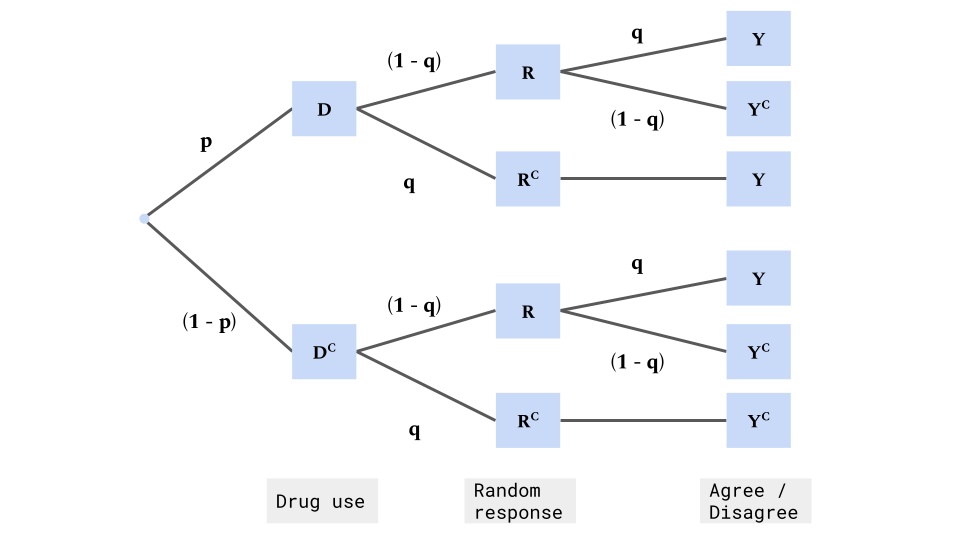
\includegraphics[width = 0.8\textwidth]{figures/probability_tree_2_a.png}
%\end{figure}
%
%\textit{Correct tree structure (may have Drug use and Random response in either order)} [1] \\
%\textit{Correct probabilities} [1] \\
%\textit{Presentation and labelling / description of `layers'} [1].
%}

b) What is the probability that a respondent replies ``Yes'' in this survey? [3]

%{\color{blue}
%\textbf{Solution:}
%
%By the law of total probability
%\begin{align*}
%\Pr(Y) =  \Pr(Y | D \cap R^C) \Pr(D \cap R^C) &+   \Pr(Y | D \cap R) \Pr(D \cap R) +  \\
%	      \Pr(Y | D^C \cap R^C) \Pr(D^C \cap R^C) &+   \Pr(Y | D^C \cap R) \Pr(D^C \cap R).
%\end{align*}
%%
%Since response randomisation is independent of whether the student has taken drugs we have that 
%\begin{align*}
%\Pr(Y) = \Pr(Y | D \cap R^C) \Pr(D) \Pr(R^C) &+ \Pr(Y | D \cap R) \Pr(D) \Pr(R) +  \\
%             \Pr(Y | D^C \cap R^C) \Pr(D^C) \Pr(R^C) &+ \Pr(Y | D^C \cap R) \Pr(D^C) \Pr(R).
%\end{align*}
%%
%Substituting the given probabilities:
%%
%\begin{align*}
%\Pr(Y) &= 1pq + q p (1 - q) + 0(1-p)q + q(1-p)(1-q) \\
%       &= pq + p(1-q)q + (1-p)(1-q)q \\
%       & = q( p + 1 - q ).
%\end{align*}
%
%\textit{correct answer} [1] \\
%\textit{correct working} [1] \\
%\textit{description / justification of steps} [1].
%}

c) Janine replied ``Yes'' in the survey. What is the probability that she had not taken performance enhancing drugs? [2]

%{\color{blue}
%\textbf{Solution:}
%%
%\begin{align*}
%    \Pr(D^C | Y) &= \frac{\Pr(D^C \cap Y)}{\Pr(Y)} \\[1.5em]
%                 &= \frac{(1-p)(1-q)q}{pq + p(1-q)q + (1-p)(1-q)q} \\[1.5em]
%                 &= \frac{(1-p)(1-q)}{p + p(1-q) + (1-p)(1-q)} \\[1.5em]
%                 &= \frac{(1-p)(1-q)}{p + 1 - q}.
%\end{align*}
%
%\textit{Working} [1] \\
%\textit{Answer} [1]
%}

d) By equating the sample and population proportions of respondents answering ``Yes'', derive the method of moments estimator $\hat P$ for $p$ based on $n$ responses to this survey design. In your derivation, denote the survey responses $Y_1, Y_2, \ldots, Y_n$ where $Y_i = 1$ if the student answered ``Yes'' and $Y_i = 0$ if the student answered ``No''. Let the mean of these responses be $\bar Y$. [2]

%{\color{blue}
%\textbf{Solution:}
%%
%We previously showed that $ \Pr(Y) = q [p + 1 - q]$. Rearranging this expression for $p$ we find that: 
%
%$$ p = \frac{\Pr(Y)}{q} - 1 + q.$$ 
%
%Replacing $\Pr(Y)$ by its method of moments estimator $\bar Y$, we obtain a method of moments estimator for $p$:
%
%$$ \hat P = \frac{\bar Y}{q} - 1 + q.$$
%
%\textit{Correct and justified working } [1] \\
%\textit{Correct answer} [1] 
%}

e) Explain why values of  0 and 1 for $q$ would not be suitable in this survey design. [2]

%{\color{blue}
%\textbf{Solution:}
%%
%Firstly, setting $q = 1$ would not be suitable because then all students would answer honestly, defeating the aim of providing responding students with plausible deniability. [1] (1 mark for valid reasoning)
%
%Secondly, setting $q = 0$ would cause at least two issues:  the first of these is that all students would respond randomly and we would gain no useful information about the proportion of students taking study drugs. Secondly, the estimator $\hat P$ is not well defined when $q = 0$. [1] (1 mark for one or more valid reasons)
%}

f)  For which values of $q$ does the method of moments estimate $\hat p$ yield a valid probability? Why is it challenging to select $q$ to satisfy this condition? [2] 

%{\color{blue}
%\textbf{Solution:}
%%
%To ensure the estimate $\hat p$ is a valid probability it must be in the range [0,1]. To ensure that this is the case we must select $q$ such that $0 \leq \frac{\bar y}{q} - 1 + q \leq 1$. [1]
%
%Enforcing this constraint is non-trivial because the value for $q$ is selected before the survey is taken, and so $\hat y$ is unknown.  (This is further complicated by the fact that the distribution of $\hat Y$ depends  on both the unknown, true proportion $p$ and the value that will be chosen for $q$.) [1] 
%
%(1 mark for condition, 1 mark for valid reasoning)
%}


g) Of the 150 students surveyed using the randomised response survey design using q = 0.4, 99 students responded ``No'''. Calculate a point estimate for the proportion of students who have taken performance enhancing drugs this exam season. [2]

%{\color{blue}
%\textbf{Solution:}
%%
%Using this survey data $\hat \Pr(Y) = 1 - \frac{99}{150} = \frac{51}{150}$ and
%
%$$ \hat p = \frac{51}{150 \times \frac{4}{10}} - 1 + \frac{4}{10} = \frac{51}{60} - \frac{36}{60} = \frac{1}{4} . $$
%
%Therefore, based on this survey, our best estimate for the proportion of students using performance enhancing drugs is $25\%$. 
%
%\textit{Correct working and justification} [1]  \\
%\textit{Correct answer, given in context} [1]
%}

\section{Ethical AI in Social Media [10] }

A social media company collects information about its users and their browsing history. The company use this information to construct and deploy an automated system that suggests future content and advertisements to each user based on their characteristics and previous activity.  

In this context, briefly explain each of the five principles of ethical AI as given in ``A unified framework of five principles for AI in society'' (Floridi and Cowls 2019)  and give an example of what each could mean in practical terms. [10] 
%{\color{blue}
%\textbf{Solution:} \textit{1 mark for definition and 1 mark for correct example \textbf{in context} for each principle: beneficence, non-maleficence, autonomy, justice and explainability.}
%
%%---------------
%\vspace{2em}
%
%\hrule 
%
%\vspace{2em}
%%---------------
%
%\textbf{Beneficence:  Promoting Well-Being, Preserving Dignity, and Sustaining the Planet} 
%
%\textit{Principle:} The use of the recommender system should benefit the user, society or the environment in some way. [1]
%
%\textit{Example context:} Recommended content might be more relevant to that user than generic recommendations, the system may also raise awareness of social or environmental issues.  [1]
%
%
%\textbf{Non-maleficence: Privacy, Security and ‘Capability Caution’}
%
%\textit{Principle:} The use of the recommender system should not cause harm to individual users, society or the environment. [1]
%
%\textit{Example context:} The recommender system should not produce echo-chambers, where users are not exposed to opinions and beliefs that contradict their own, thereby leading to a more polarised society. [1]
%
%
%\textbf{Autonomy: The Power to Decide (to Decide)} 
%
%\textit{Principle:} The use of the recommender system should not impair the freedom of human beings to set their own standards and norms. [1]
%
%\textit{Example context:} Humans, whether staff members of the social media company or users, should be able to intervene and over-ride the recommendations made by e.g. turning off all tailored content or `muting' topics such as maternity content. [1]
%
%
%\textbf{Justice: Promoting Prosperity, Preserving Solidarity, Avoiding Unfairness} 
%
%\textit{Principle:} The use of the recommender system should seek to eliminate existing injustice and discrimanation and to provide equitable access to the benefits of the system. [1]
%
%\textit{Example context:} The recommendations made should be equitable across all members of society, this could fail if skin-tone biases or Eurocentric beauty standards are exacerbated by the recommendations made by the system. [1]
%
%
%\textbf{Explicability:}
%
%\textit{Principle:} Users who are not experts in recommender systems should be able to understand why they are being shown certain content. [1]
%
%\textit{Example context:} Personalised content might be displayed with a message such as `users who follow X also follow Y', or 'because you liked Z ...'. [1]
%}
\end{document}